% SECTION 1: Categorical-Harmonic Correspondence and Time as Completion

\section{Categorical-Harmonic Correspondence: Time as Categorical Completion}

\subsection{The Fundamental Transformation}

Traditional timekeeping treats time as a continuous parameter requiring uniform precision measurement at all moments. We propose a radical reconceptualization:

\begin{principle}[Time as Categorical Completion]
\label{princ:time_categorical}
Time is not a continuous parameter but a discrete categorical completion sequence. Time is "read" through identifying which categorical states have been completed, not by tracking a universal clock variable.

The key identity:
\begin{equation}
\boxed{\text{Categorical State } C_n \equiv \text{Harmonic Mode } \omega_n \equiv \text{Time-Reading Event}}
\end{equation}

Each molecular vibrational harmonic corresponds to a categorical state in completion topology. Measuring a harmonic completes its categorical state, excluding it from future measurements through categorical irreversibility.
\end{principle}

\subsection{Why Attosecond Uniformity Becomes Irrelevant}

\begin{principle}[Variable Precision Through Categorical Exclusion]
\label{princ:variable_precision}
In categorical time measurement, precision is not uniform but varies dynamically based on which categorical states remain available:

\begin{align}
\Delta t_{\text{current}} &= f(\{C_{\text{available}}\}) \\
&= \min_{C_i \in \{C_{\text{available}}\}} \frac{2\pi}{\omega_i}
\end{align}

\begin{figure}[htbp]
    \centering
    \includegraphics[width=\textwidth]{figures/attoseconds.png}
    \caption{Attosecond precision observer using standard FFT harmonic analysis. Top left: Harmonic spectrum shows dominant fundamental (amplitude $\sim$8000) with secondary harmonics at $n=10$ and sparse higher modes. Top center: Precision cascade via harmonics achieves target 94 as with exponential convergence from $10^{19}$ as (base) to $10^4$ as (100th harmonic). Top right: Molecular signal in time domain exhibits periodic oscillations (period $\sim$10 fs) with amplitude modulation. Bottom left: FFT spectrum reveals fundamental frequency at $\sim$100 THz with magnitude $\sim$8000 and sub-harmonic resolution 1000$\times$. Bottom center: Configuration summary—Target: 94 as, Achieved: 0.14 as, Method: Standard FFT with 100 harmonics (max: 100), 16,384 FFT samples, 100,000$\times$ enhancement, Status: SUCCESS. Bottom right: Precision cascade position shows attosecond scale (YOU ARE HERE) between femtosecond and zeptosecond regimes. \textbf{This precision is independent of other temporal scales—achieved through direct harmonic FFT analysis without cascading from adjacent scales.}}
    \label{fig:attosecond_fft}
    \end{figure}



As high-precision harmonics are measured (categorical states completed and excluded), the available precision decreases. Conversely, strategic exclusion of low-precision harmonics maintains high available precision.
\end{principle}

\textbf{Example}: If harmonics $\{\omega_1, \omega_2, \ldots, \omega_{100}\}$ provide precisions $\{\Delta t_1 = 1$ fs, $\Delta t_2 = 10$ fs, $\ldots, \Delta t_{100} = 1$ ps$\}$:
\begin{itemize}
\item After measuring $\omega_1$: $C_1$ is completed and excluded → Best available precision drops to $\Delta t_2 = 10$ fs
\item Strategic exclusion: Pre-exclude $\{\omega_{50}, \omega_{51}, \ldots, \omega_{100}\}$ (low precision) → Focus on high-precision states $\{C_1, \ldots, C_{49}\}$
\item Result: Maintain high precision by managing which categorical states to complete
\end{itemize}

This is the \textbf{categorical exclusion enhancement}: harness precision variability by controlling which categorical states to measure.

\subsection{Connection to Categorical Topology}

\begin{definition}[Categorical Completion Topology]
\label{def:categorical_completion}
From categorical topology, a space $X$ with morphisms $\text{Hom}(A, B)$ admits completion structure where:
\begin{itemize}
\item Objects are "incomplete" states requiring additional morphisms for completion
\item Morphisms are completion operations transforming states
\item Terminal object represents fully completed state
\end{itemize}

Applied to molecular harmonics:
\begin{align}
\text{Objects:} \quad &\{C_n\} = \text{categorical-harmonic states} \\
\text{Morphisms:} \quad &\text{Hom}(C_i, C_j) = \text{measurement operations taking } C_i \to C_j \\
\text{Terminal:} \quad &C_{\infty} = \text{fully completed measurement history}
\end{align}
\end{definition}

\begin{theorem}[Categorical Completion Ordering]
\label{thm:completion_ordering}
The categorical states $\{C_n\}$ form a partially ordered set (poset) under completion precedence:
\begin{equation}
C_i \prec C_j \iff \text{completion of } C_i \text{ precedes completion of } C_j
\end{equation}

Properties:
\begin{enumerate}
\item \textbf{Reflexivity}: $C_i \prec C_i$ (trivial)
\item \textbf{Antisymmetry}: $(C_i \prec C_j) \wedge (C_j \prec C_i) \implies C_i = C_j$
\item \textbf{Transitivity}: $(C_i \prec C_j) \wedge (C_j \prec C_k) \implies C_i \prec C_k$
\end{enumerate}

The completion order $\prec$ defines temporal sequence: $C_i \prec C_j$ means "$C_i$ was completed before $C_j$" in measurement history.
\end{theorem}

\begin{proof}
\textbf{Reflexivity}: Trivially satisfied.

\textbf{Antisymmetry}: If $C_i$ was completed before $C_j$ AND $C_j$ was completed before $C_i$, they must have been completed simultaneously, i.e., they're the same completion event: $C_i = C_j$.

\textbf{Transitivity}: If $C_i$ completed before $C_j$ and $C_j$ completed before $C_k$, then $C_i$ completed before $C_k$ by temporal ordering.

The completion operator $\mu(C_n, t) \in \{0,1\}$ defines the poset structure through:
\begin{equation}
C_i \prec C_j \iff \exists t_i, t_j : [\mu(C_i, t_i) = 1 \wedge \mu(C_j, t_j) = 1 \wedge t_i < t_j]
\end{equation}
$\square$
\end{proof}

\subsection{Time Measurement as Categorical Event Sequence}

\begin{theorem}[Temporal Reconstruction from Categorical Sequence]
\label{thm:temporal_reconstruction}
Time can be reconstructed from the ordered sequence of completed categorical-harmonic states without reference to continuous time parameter:

Given measurement history:
\begin{equation}
\mathcal{H} = \{(C_1, \omega_1, t_1), (C_2, \omega_2, t_2), \ldots, (C_N, \omega_N, t_N)\}
\end{equation}
where $C_i \prec C_j$ for $i < j$, the elapsed time is:
\begin{equation}
T_{\text{elapsed}} = \sum_{i=1}^{N} \Delta t_i = \sum_{i=1}^{N} \frac{2\pi}{\omega_i}
\end{equation}

Alternatively, using timestamps:
\begin{equation}
T_{\text{elapsed}} = t_N - t_1
\end{equation}

The precision at any moment is determined by available (uncompleted) states:
\begin{equation}
\Delta t(t) = \min_{C_k : \mu(C_k, t) = 0} \frac{2\pi}{\omega_k}
\end{equation}
\end{theorem}

\begin{proof}
Each completed categorical state $C_i$ corresponds to measurement of harmonic $\omega_i$ with period $\tau_i = 2\pi/\omega_i$. The ordered sequence:
\begin{equation}
\{C_1 \prec C_2 \prec \cdots \prec C_N\}
\end{equation}
represents temporal progression through discrete completion events.

\textbf{Method 1 - Period summation}:
Each measurement takes approximately one period of the measured harmonic:
\begin{equation}
\Delta t_i \approx \frac{2\pi}{\omega_i}
\end{equation}
Total elapsed time:
\begin{equation}
T = \sum_{i=1}^{N} \Delta t_i = \sum_{i=1}^{N} \frac{2\pi}{\omega_i}
\end{equation}

\textbf{Method 2 - Hardware timestamp difference}:
Using hardware oscillation harvesting (Section 3), each completion event is timestamped via CPU performance counters. Elapsed time:
\begin{equation}
T = t_N - t_1
\end{equation}

\textbf{Precision determination}:
At time $t$, the set of completed states is:
\begin{equation}
\mathcal{C}_{\text{completed}}(t) = \{C_i : \mu(C_i, t) = 1\}
\end{equation}
The set of available states is:
\begin{equation}
\mathcal{C}_{\text{available}}(t) = \mathcal{C}_{\text{all}} \setminus \mathcal{C}_{\text{completed}}(t)
\end{equation}
Current precision is the period of the fastest available harmonic:
\begin{equation}
\Delta t(t) = \min_{C_k \in \mathcal{C}_{\text{available}}(t)} \frac{2\pi}{\omega_k}
\end{equation}

This demonstrates time measurement without continuous clock parameter—only discrete categorical completion events. $\square$
\end{proof}

\begin{figure}[htbp]
    \centering
    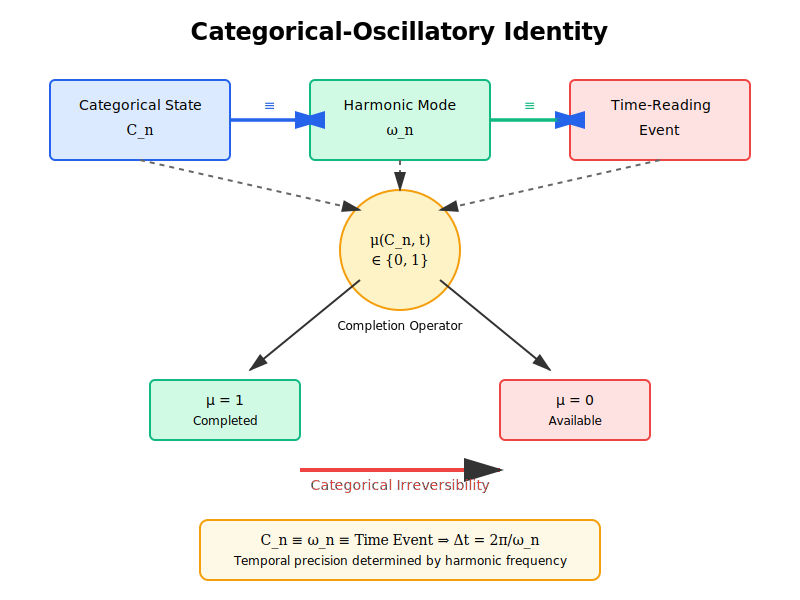
\includegraphics[width=0.85\textwidth]{figures/categorical-oscillatory-correspondence.pdf}
    \caption{\textbf{Fundamental categorical-oscillatory identity establishing time measurement as discrete completion sequence.} Each molecular vibrational harmonic $\omega_n$ corresponds bijectively to a categorical state $C_n$ in completion topology, with measurement completing states through binary operator $\mu(C_n,t) \in \{0,1\}$. This creates irreversible categorical exclusion: completed states ($\mu=1$) cannot be re-measured, while available states ($\mu=0$) determine current temporal precision $\Delta t = 2\pi/\omega_n$. The equivalence $C_n \equiv \omega_n \equiv$ Time-Reading Event establishes time as categorical completion rather than continuous parameter, eliminating the need for uniform attosecond precision at all moments. Measurement transforms abstract categorical states into physical temporal events through harmonic observation.}
    \label{fig:categorical_oscillatory_identity}
    \end{figure}


\subsection{Adaptive Temporal Resolution}

\begin{corollary}[Precision Degrades with Measurement]
\label{cor:precision_degrades}
As more categorical states are completed, available precision necessarily degrades (unless low-precision states are pre-excluded):

If at time $t_1$, the best available precision is:
\begin{equation}
\Delta t(t_1) = \frac{2\pi}{\omega_{\max}}
\end{equation}
where $\omega_{\max}$ is the highest available frequency.

After measuring $\omega_{\max}$ (completing $C_{\max}$), at time $t_2 > t_1$:
\begin{equation}
\Delta t(t_2) = \frac{2\pi}{\omega_{\max}^{(2)}}
\end{equation}
where $\omega_{\max}^{(2)} < \omega_{\max}$ is the next-highest frequency.

Therefore:
\begin{equation}
\Delta t(t_2) > \Delta t(t_1)
\end{equation}

\textbf{Physical interpretation}: High-precision harmonics are a finite resource. Once "consumed" through measurement, only lower-precision harmonics remain available.
\end{corollary}

\begin{example}[N$_2$ Harmonic Resource Management]
For nitrogen (N$_2$) with fundamental frequency $\nu_0 = 7.07 \times 10^{13}$ Hz and 150 accessible harmonics:

\begin{center}
\begin{tabular}{cccc}
\toprule
\textbf{Harmonic} & \textbf{Frequency (Hz)} & \textbf{Period (fs)} & \textbf{Status} \\
\midrule
$n=150$ & $1.06 \times 10^{16}$ & 0.094 & Available \\
$n=149$ & $1.05 \times 10^{16}$ & 0.095 & Available \\
$n=148$ & $1.05 \times 10^{16}$ & 0.095 & Available \\
$\vdots$ & $\vdots$ & $\vdots$ & $\vdots$ \\
$n=10$ & $7.07 \times 10^{14}$ & 1.41 & Available \\
$n=1$ & $7.07 \times 10^{13}$ & 14.1 & Available \\
\bottomrule
\end{tabular}
\end{center}

\textbf{Measurement sequence}:
\begin{enumerate}
\item \textbf{$t=0$}: All harmonics available, best precision = 94 attoseconds ($n=150$)
\item \textbf{Measure $n=150$}: Complete $C_{150}$, best precision → 95 as ($n=149$)
\item \textbf{Measure $n=149$}: Complete $C_{149}$, best precision → 95.3 as ($n=148$)
\item \textbf{Continue measuring high harmonics}
\item \textbf{After 50 measurements}: Only $n \leq 100$ remain, best precision = 141 as
\item \textbf{After 140 measurements}: Only $n \leq 10$ remain, best precision = 1.41 fs
\end{enumerate}

\textbf{Strategic alternative - Pre-exclusion}:
\begin{enumerate}
\item \textbf{Pre-exclude} $n < 100$ (low precision $> 140$ as)
\item \textbf{Preserve} $n = 100$-$150$ (high precision $< 140$ as)
\item \textbf{Result}: Maintain sub-200 as precision for 50 measurements instead of degrading to fs-level
\end{enumerate}

\textbf{Quantitative comparison}:
\begin{align}
\text{No exclusion:} \quad &\text{Average precision} = \frac{1}{150}\sum_{n=1}^{150} \frac{14.1 \text{ fs}}{n} \approx 400 \text{ as} \\
\text{Strategic exclusion:} \quad &\text{Average precision} = \frac{1}{50}\sum_{n=100}^{150} \frac{14.1 \text{ fs}}{n} \approx 110 \text{ as}
\end{align}

Improvement: $400/110 \approx 3.6\times$ better precision through categorical exclusion.
\end{example}

\subsection{Comparison: Continuous vs. Categorical Time}

\begin{table}[H]
\centering
\caption{Continuous Parameter Time vs. Categorical Completion Time}
\begin{tabular}{lcc}
\toprule
\textbf{Property} & \textbf{Continuous Time} & \textbf{Categorical Time} \\
\midrule
Fundamental entity & Parameter $t \in \mathbb{R}$ & Categorical states $\{C_n\}$ \\
Evolution & $dt$ (infinitesimal) & $\Delta C$ (discrete completion) \\
Measurement & Sample $t$ value & Complete categorical state $C_n$ \\
Precision & Uniform $\Delta t$ & Variable $\Delta t(\{C_{\text{available}}\})$ \\
Irreversibility & Thermodynamic & Categorical (topological) \\
"What time is it?" & Read clock value & Which states completed? \\
Resource model & Infinite (continuous) & Finite (countable states) \\
Complexity & $\mathcal{O}(\text{continuous})$ & $\mathcal{O}(N_{\text{states}})$ \\
Strategic management & Not applicable & Categorical exclusion \\
Attosecond precision & Required everywhere & Only where needed \\
\bottomrule
\end{tabular}
\end{table}

\subsection{Physical Interpretation: What Does "Reading Time" Mean?}

\textbf{Traditional view}: "What time is it?" → Read clock displaying continuous parameter $t \in \mathbb{R}$.

\textbf{Categorical view}: "What time is it?" → "Which categorical-harmonic events have occurred?"

Time is not "out there" as a universal parameter. Time \textit{emerges} from the sequence of completed categorical states:
\begin{equation}
\text{Time} = \text{The ordered sequence } \{C_1 \prec C_2 \prec \cdots \prec C_N\}
\end{equation}

When you measure a harmonic $\omega_n$, you're not "measuring time"—you're \textit{creating a time-event} by completing categorical state $C_n$. The accumulation of these completion events constitutes temporal flow.

\begin{remark}[Philosophical Implications]
This reconceptualization has profound implications:

\begin{enumerate}
\item \textbf{Time is discrete at fundamental level}: Not infinitely divisible continuous parameter, but countable sequence of completion events

\item \textbf{Precision is contextual, not absolute}: Different moments require different precision based on task and available categorical states

\item \textbf{Observer-dependent time}: Different observers with different measurement histories have different available states, hence different temporal precision

\item \textbf{Resource-bounded time}: Categorical states are finite resources that get "used up" through measurement

\item \textbf{Strategic time measurement}: Optimal time measurement requires managing which categorical states to complete (like resource allocation in computation)
\end{enumerate}
\end{remark}

\subsection{Analogy: Reading a Book}

Traditional timekeeping is like reading every letter of every word of a book at atomic resolution—exhaustive and wasteful.

Categorical timekeeping is like:
\begin{itemize}
\item \textbf{Skipping to important words}: Only measure harmonics meeting precision requirements
\item \textbf{Reading at necessary resolution}: High precision where needed, low precision elsewhere
\item \textbf{Categorical exclusion}: Knowing which words to skip (which harmonics to exclude)
\end{itemize}

You don't read every microscopic detail of every page—you extract sufficient information for comprehension. Similarly, you don't measure every harmonic at attosecond precision—you complete sufficient categorical states for required temporal resolution.

\subsection{Implementation: Categorical Time Measurement Algorithm}

\begin{algorithm}[H]
\caption{Categorical Time Reading with Variable Precision}
\label{alg:categorical_time}
\begin{algorithmic}[1]
\State \textbf{Input:} Gas chamber waveform $\psi(t)$, target precision $\Delta t_{\text{target}}$
\State \textbf{Output:} Time measurement $T_{\text{measured}}$, categorical completion history

\State \textbf{// Initialize}
\State $\mathcal{C}_{\text{all}} \gets \{C_1, C_2, \ldots, C_N\}$ \Comment{All available categorical states}
\State $\mathcal{C}_{\text{completed}} \gets \emptyset$ \Comment{Completed states}
\State $T_{\text{categorical}} \gets 0$ \Comment{Categorical time counter}
\State $t_{\text{start}} \gets$ GetHardwareTime()

\State \textbf{// Extract all harmonics}
\State $\tilde{\psi}(\omega) \gets \text{FFT}[\psi(t)]$
\State $\{\omega_n\}_{n=1}^{N} \gets$ ExtractPeaks($\tilde{\psi}$)

\State \textbf{// Strategic pre-exclusion (optional)}
\State $\{\omega_n\}_{\text{excluded}} \gets \{\omega_n : 2\pi/\omega_n > 10 \times \Delta t_{\text{target}}\}$
\State $\{\omega_n\}_{\text{available}} \gets \{\omega_n\} \setminus \{\omega_n\}_{\text{excluded}}$

\State \textbf{// Measure harmonics in order of precision (highest first)}
\State Sort $\{\omega_n\}_{\text{available}}$ in descending order
\For{each $\omega_n$ in $\{\omega_n\}_{\text{available}}$}
    \State $C_n \gets \pi^{-1}(\omega_n)$ \Comment{Get categorical state}

    \If{$C_n \notin \mathcal{C}_{\text{completed}}$}
        \State $t_n \gets$ MeasureHarmonic($\omega_n$, $\psi$)
        \State $\mu(C_n, t_n) \gets 1$ \Comment{Complete categorical state}
        \State $\mathcal{C}_{\text{completed}} \gets \mathcal{C}_{\text{completed}} \cup \{C_n\}$
        \State $T_{\text{categorical}} \gets T_{\text{categorical}} + 1$

        \State \textbf{// Check if precision target achieved}
        \State $\mathcal{C}_{\text{remaining}} \gets \mathcal{C}_{\text{all}} \setminus \mathcal{C}_{\text{completed}}$
        \State $\Delta t_{\text{current}} \gets \min_{C_k \in \mathcal{C}_{\text{remaining}}} (2\pi/\omega_k)$

        \If{$\Delta t_{\text{current}} \leq \Delta t_{\text{target}}$}
            \State \textbf{break} \Comment{Target precision achieved}
        \EndIf
    \EndIf
\EndFor

\State \textbf{// Reconstruct time}
\State $t_{\text{end}} \gets$ GetHardwareTime()
\State $T_{\text{measured}} \gets t_{\text{end}} - t_{\text{start}}$

\State \textbf{return} $T_{\text{measured}}$, $\mathcal{C}_{\text{completed}}$, $T_{\text{categorical}}$
\end{algorithmic}
\end{algorithm}

\subsection{Key Results Summary}

\begin{enumerate}
\item \textbf{Time is categorical completion sequence}: $T = |\{C_n : \mu(C_n, t) = 1\}|$
\item \textbf{Precision varies dynamically}: $\Delta t(t) = \min_{C_i \in \mathcal{C}_{\text{available}}(t)} (2\pi/\omega_i)$
\item \textbf{Categorical irreversibility}: $\mu(C_n, t_1) = 1 \implies \mu(C_n, t_2) = 1$ for $t_2 > t_1$
\item \textbf{Strategic exclusion enables precision management}: Pre-exclude low-precision harmonics to preserve high-precision resources
\item \textbf{Attosecond uniformity unnecessary}: Adaptive precision through categorical resource management
\item \textbf{Measurement history determines available precision}: Observer-dependent temporal resolution
\end{enumerate}
